%-------------------------------PPT Title-------------------------------------
\title{}
%-----------------------------------------------------------------------------

%----------------------------Author & Date------------------------------------
\author[]{姜\;\;骏\inst{}} %[]{} (optional, use only with lots of authors)
% - Give the names in the same order as the appear in the paper.
% - Use the \inst{?} command only if the authors have different
%   affiliation.
\institute[BCC]{\inst{}%
 \vskip -30pt 北京市计算中心\;云平台事业部}
\date[\today] % (optional, should be abbreviation of conference name)
{%	{\fontsize{6.2pt}{4.2pt}\selectfont{\textcolor{blue}{E-mail:~}\url{jiangjun@bcc.ac.cn}}}
\vskip 35 pt \textrm{2024.09.03}
%\vskip 5 pt {\fontsize{8.2pt}{6.2pt}\selectfont{清华大学\;\;材料学院}}
}

% - Either use conference name or its abbreviation
% - Not really information to the audience, more for people (including
%   yourself) who are reading the slides online

%\subject{}
% This is only inserted into the PDF information catalog. Can be left
%\frame
%{	
%	\frametitle{\footnotesize{\textcolor{orange}{\textrm{2018~}年度北京市计算中心职称评聘答辩}}}
%\titlepage
%}
%-----------------------------------------------------------------------------
%\maketitle
%------------------------------------------------------------------------------列出全文 outline ---------------------------------------------------------------------------------
%\section*{}
%\frame[allowframebreaks]
%{
%  \frametitle{Outline}
%  \frametitle{\textcolor{mycolor}{\secname}}
%  \tableofcontents%[current,currentsection,currentsubsection]
%}
%在每个section之前列出全部Outline
%类似的在每个subsection之前列出全部Outline是\AtBeginSubsection[]
%\AtBeginSection[]
%{
%  \frame<handout:0>
%  {
%    \frametitle{Outline}
%%全部Outline中,本部分加亮
%    \tableofcontents[current,currentsection]
%  }
%}

%------------------------------------------------------------------------------PPT main Body------------------------------------------------------------------------------------
\small
%\section{个人信息}
\frame
{
	\frametitle{个人信息}
	\vskip -35pt
\begin{minipage}[b]{0.72\linewidth}
	\fontsize{9.2pt}{6.2pt}\selectfont{姓~名\hspace{15pt}姜~骏\hspace{45pt}出生年月\hspace{15pt}\textrm{1978.12}}\\
	\vskip 7pt
	学~位\hspace{15pt}理学博士\hspace{29pt}专业方向\hspace{15pt}物理化学\\
	\vskip 7pt
	\fontsize{8.2pt}{6.2pt}\selectfont{工作部门\hspace{5pt}北京市计算中心~云平台事业部}\\
\end{minipage}
\hfill
\begin{minipage}[b]{0.26\linewidth}
	\vspace{40pt}
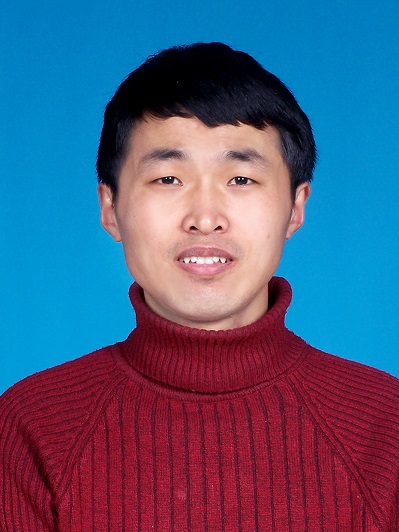
\includegraphics[height=0.7in]{Figures/Person_Photo.JPG}
\end{minipage}\vskip 3pt
\fontsize{9.2pt}{6.2pt}\selectfont{\textcolor{magenta}{教育背景}}
	\begin{itemize}
		\item {\fontsize{8.2pt}{6.2pt}\selectfont{\textrm{2001.09-2008.01}}}~~~北京大学~化学与分子工程学院~~~~~~物理化学
		\item {\fontsize{8.2pt}{6.2pt}\selectfont{\textrm{1997.09-2001.06}}}~{\fontsize{8.2pt}{6.2pt}\selectfont{中国纺织大学(现~东华大学)}}~{\fontsize{8.2pt}{6.2pt}\selectfont{纺织化学系~染整工程}}
	\end{itemize}
	\fontsize{9.2pt}{6.2pt}\selectfont{\textcolor{magenta}{工作简历}}
\begin{minipage}{\textwidth}
\begin{table}[!h]
\tabcolsep 0pt %\vspace*{-5pt}
%\caption{经费预算表 (单位:~万元).}
\label{Table-Cost}
%\begin{center}
\centering
\def\temptablewidth{0.94\textwidth}
\renewcommand\arraystretch{2.2} %表格宽度控制(普通表格宽度的两倍)
\rule{\temptablewidth}{1pt}
\begin{tabular*} {\temptablewidth}{@{\extracolsep{\fill}}c@{\extracolsep{\fill}}c@{\extracolsep{\fill}}c}
%-------------------------------------------------------------------------------------------------------------------------
	起止时间 &工作单位	&研发岗位 \\\hline
	\fontsize{8.2pt}{6.2pt}\selectfont{\textrm{2008.01-2012.03}} &\fontsize{8.2pt}{6.2pt}\selectfont{北京大学~化学与分子工程学院} &\fontsize{8.2pt}{6.2pt}\selectfont{博士后} \\
	\fontsize{8.2pt}{6.2pt}\selectfont{\textrm{2012.03-2013.03}} &\fontsize{8.2pt}{6.2pt}\selectfont{北京宏剑公司} &\fontsize{8.2pt}{6.2pt}\selectfont{高级技术支持}\\
	\fontsize{8.2pt}{6.2pt}\selectfont{\textrm{2013.04-2016.03}} &\fontsize{7.8pt}{6.2pt}\selectfont{中物院高性能数值模拟软件中心} &\fontsize{8.2pt}{6.2pt}\selectfont{金属材料模拟团队} \\
	\fontsize{8.2pt}{6.2pt}\selectfont{\textrm{2016.04-至今}}    &\fontsize{8.2pt}{6.2pt}\selectfont{北京市计算中心} &\fontsize{8.2pt}{6.2pt}\selectfont{云平台事业部}\\
\end{tabular*}
\rule{\temptablewidth}{1pt}
%\end{center}
\end{table}
%\vskip -3pt
\end{minipage}
}

\begin{frame}
	\frametitle{研究方向、承担项目和成果}
	{\fontsize{8.2pt}{6.2pt}\selectfont{长年从事基于密度泛函理论(\textrm{DFT})的第一原理计算方法、算法和软件及其应用(微观材料计算与模拟)研究,对分子动力学~(\textrm{MD})方法有所涉猎}}
\vskip 5pt
	\textcolor{blue}{2016年起,将数据挖掘、知识图谱、人工智能相关的机器学习算法,特别是人工神经网络算法应用到第一原理和分子动力学材料研究的软件开发和模拟计算中,对相关方法、算法有全面的认识}
\begin{itemize}
	\setlength{\itemsep}{5pt}
	\item {\fontsize{8.2pt}{6.2pt}\selectfont{国家重点研发计划项目~(本单位任务责任人)}}:\\
		“高通量并发式材料计算算法和软件”~{\fontsize{8.2pt}{6.2pt}\selectfont{(已结题)}}
	\item {\fontsize{8.2pt}{6.2pt}\selectfont{“新材料研发及应用”国家重大专项(科技创新2030重大项目)}}:\\
		“基于人工智能技术的高性能多尺度分子动力学模拟平台”
	\item {\fontsize{8.2pt}{6.2pt}\selectfont{国家自然科学基金~(本单位项目责任人)}}:\\
		“低维材料等离和激子极化激元的第一性原理研究”
\end{itemize}
{\fontsize{8.5pt}{7.0pt}\selectfont{\centering \textcolor{purple}{发表论文6篇,获得发明专利1项、软著2项、参与编著专著1本,论文6篇}}}
\end{frame}

%\appendix
%\frame
%{
%	\frametitle{学术积累}
%\textcolor{magenta}{发表论文}
%	\begin{itemize}
%		\item {\fontsize{5.2pt}{1.2pt}\selectfont{\textrm{Yang Ge, Jianlong Ji, Zhizhong Shen, Qiang Zhang, Aoqun Jian, Qianqian Duan, Chao Wang, \underline{Jun Jiang}, Wendong Zhang, Shengbo Sang, First principles study of magnetism induced by topological frustration of bowtieshaped graphene nanoflake, \textit{Carbon}, \textbf{127}, (2018), 432-436}}}
%		\item {\fontsize{5.2pt}{1.2pt}\selectfont{\textrm{\underline{JIANG Jun}, BIAN Jiang; LI Le-Min, Theoretical Assignments of the Optical Conductivity and Energy-loss Function Spectra of EuB$_6$, \textit{Acta Physico-Chimica Sinica}, \textbf{24}, (2008), 1-7}}}
%	\end{itemize}
%}
